\documentclass[a4paper,10pt]{article}

\usepackage[hidelinks]{hyperref}
\usepackage{float}
\usepackage{tabularx}

% Lingua 
\usepackage[utf8]{inputenc}
\usepackage[italian]{babel}

% Margini
\usepackage{geometry}
\geometry{a4paper, top=3cm, bottom=3cm, left=3cm, right=3cm}
\setlength{\parindent}{0pt}

\usepackage{graphicx}   % per immagini
\usepackage{caption}    % per didascalie
\captionsetup[table]{labelformat=empty}
\usepackage{ifthen}     % per \ifthenelse
\usepackage{longtable}

\usepackage{array}      % per tabelle
\newcolumntype{M}[1]{>{\centering\arraybackslash}m{#1}}

\setcounter{secnumdepth}{5}
\setcounter{tocdepth}{5}
\usepackage{titlesec}

\titleformat{\paragraph}[block]  % <-- QUESTO è il punto chiave
  {\normalfont\normalsize\bfseries}
  {\theparagraph}
  {1em}
  {}

\titlespacing*{\paragraph}
  {0pt}
  {3ex}
  {1.5ex}

\usepackage{datetime}

% Definisci un formato personalizzato
\newdateformat{italianformat}{\THEDAY~\monthname[\THEMONTH]~\THEYEAR}
\newdate{dataverbale}{02}{04}{2026}

% Definizione del formato con le barre
\newdateformat{slashdate}{\twodigit{\THEDAY}/\twodigit{\THEMONTH}/\THEYEAR}

% Per logo in ogni pagina
\usepackage{eso-pic}
\usepackage{tikz}
\AddToShipoutPictureBG{%
  \ifthenelse{\value{page}>1}{%
    \begin{tikzpicture}[remember picture, overlay]
      % Icona
      \node[anchor=north west, inner sep=0pt] at ([xshift=28pt,yshift=-28pt]current page.north west) 
        {
\includegraphics[width=1cm, height=1cm]{resources/Tool-8_icon_white.png}};
      
      % Riga
      \draw[black, line width=0.5pt] ([xshift=28pt + 1cm, yshift=-28pt - 0.6cm]current page.north west) 
            -- ++(3.2cm, 0);
      % Testo
      \node[anchor=west, text=black, font=\small] at ([xshift=28pt + 1cm, yshift=-28pt - 0.4cm]current page.north west) 
        {Specifica Tecnica};
    \end{tikzpicture}
  }{}
}

% Nome indice figure
\addto\captionsitalian{%
  \renewcommand{\listfigurename}{Indice delle immagini}%
}


%------Ridefinizione maketitle-------
\makeatletter
\renewcommand{\maketitle}{%
  \vspace*{\fill}
  \begin{center}
    {\LARGE \bfseries \@title \par}
    \vskip 1em
    {\large \@author \par}
    \vskip 1em
    {\large\slashdate{\displaydate{dataverbale}} \par}
  \end{center}
  \vspace*{\fill}
}
\makeatother
%-----------------------------------

\title{%
  
\includegraphics[width=10cm]{resources/Tool-8_white_2.png} \\[1.5ex]
  \textbf{\LARGE Specifica Tecnica}
}
\author{}
\date{\dataverbale}
\begin{document}
\tikz[remember picture,overlay] \node[opacity=0.2,inner sep=0pt] at (current page.center){
\includegraphics[width=\paperwidth,height=\paperheight]{resources/Abstract_lines.png}};

\maketitle

\newpage

\section*{Revisioni}
\begin{table}[h!]
\centering
\begin{tabular}{|M{0.8cm}|p{2.2cm}|p{5.7cm}|M{1.8cm}|p{2.2cm}|}
  \hline
  \textbf{Ver.} & \textbf{Autore} & \textbf{Modifiche} & \textbf{Data} & \textbf{Verifica} \\
  \hline
  0.6 & Stefano Maso & Modifica sezione LLM & 24/04/2026 & - \\
  \hline
  0.5 & Giuliano Banchieri & Stesura sezione architettura di deployment e organizzazione container & 21/04/2026 & Spadiliero Ruben \\
  \hline
  0.4 & Stefano Maso & Aggiunte sottosezioni per l'importazione & 10/04/2026 & Besnik Murtezan \\
  \hline
  0.3 & Stefano Maso & Stesura sezione 3.1.1.2 e sottosezioni & 09/04/2026 & Besnik Murtezan \\
  \hline
  0.2 & Stefano Maso & Stesura sezione 3.1, 3.1.1 e sottosezioni relative all'architettura del backend e relativi diagrammi delle classi & 08/04/2026 & Besnik Murtezan \\
  \hline
  0.1 & Giuliano Banchieri & Prima stesura: struttura del documento, tecnologie, riferimenti, introduzione & 02/04/2026 & Niccolò Feltrin \\
  \hline
\end{tabular}
\caption{}
\label{tab:revisioni}
\end{table}

\newpage

\tableofcontents

\newpage

\listoffigures

\newpage

\section{Introduzione}
\subsection{Scopo del documento}
Il presente documento contiene informazioni dettagliate sulle tecnologie utilizzate e sulle scelte progettuali del gruppo Tool-8 per la realizzazione del prodotto \textbf{Second Brain} su richiesta dell'azienda \textbf{Zucchetti S.p.A.}

Sono fornite descrizioni delle tecnologie scelte per backend, frontend e di supporto, i diagrammi delle classi che rappresentano in modo dettagliato l'archittettura logica e una tabella di tracciamento dei requisiti soddisfatti.

\subsection{Scopo del prodotto}
"\textbf{Estendere il note-taking con i Large Language Models.}"

L'obiettivo del capitolato C6 "\textbf{Second Brain}" è lo sviluppo di un applicativo che fornisca all'utente un editor di file MD con funzionalità AI che semplifichino la scrittura tramite funzionalità come: riassunto, traduzione, critica, correzione, e generazione del testo.

L'utente avrà la possibilità di utilizzare queste funzionalità anche tramite interrogazioni in linguaggio naturale che verranno processate da un LLM contattato dal sistema.

Il software sarà sviluppato sotto forma di applicazione web dove l'utente potrà creare, salvare, eliminare e modificare le sue note.

\subsection{Riferimenti}
\subsubsection{Riferimenti normativi}
\begin{itemize}
  \item Capitolato C6 - Progetto Second Brain: \\  \url{https://www.math.unipd.it/~tullio/IS-1/2025/Progetto/C6.pdf}
  \item Regolamento progetto didattico: \\ \url{https://www.math.unipd.it/~tullio/IS-1/2025/Dispense/PD1.pdf}
  \item \href{https://tool-8.github.io/Documentazione-SWE/pb/Norme_di_Progetto_v1.1.pdf}{Norme di Progetto v1.1}
  \item \href{https://tool-8.github.io/Documentazione-SWE/pb/Analisi_dei_Requisiti_v1.5.pdf}{Analisi dei Requisiti v1.5}
\end{itemize}
\subsubsection{Riferimenti informativi}
\begin{itemize}
  \item \href{https://tool-8.github.io/Documentazione-SWE/}{Verbali}
  \item \href{https://tool-8.github.io/Documentazione-SWE/glossario/Glossario.pdf}{Glossario v1.0}
  \item Lezioni del corso di \textit{Ingegneria del software} aggiornate al 02/04/2026:
  \begin{itemize}
    \item \textit{"Progettazione software (T6)"}: \\ \url{https://www.math.unipd.it/~tullio/IS-1/2025/Dispense/T06.pdf}
    \item \textit{"Progettazione e programmazione: Diagrammi delle classi (UML)"}: \\ \url{https://www.math.unipd.it/~rcardin/swea/2023/Diagrammi%20delle%20Classi.pdf}
    \item \textit{"Analisi e descrizione delle funzionalità: Diagrammi delle attività (UML)"}: \\ \url{https://www.math.unipd.it/~rcardin/swea/2022/Diagrammi%20di%20Attivit%C3%A0.pdf}
    \item \textit{"Progettazione: I pattern architetturali"}: \\ \url{https://www.math.unipd.it/~rcardin/swea/2022/Software%20Architecture%20Patterns.pdf}
    \item \textit{"Progettazione: Il pattern Dependency Injection"}: \\ \url{https://www.math.unipd.it/~rcardin/swea/2022/Design%20Pattern%20Architetturali%20-%20Dependency%20Injection.pdf}
    \item \textit{"Progettazione: Pattern Architetturali per le applicazioni con UI"}: \\ \url{https://www.math.unipd.it/~rcardin/sweb/2022/L02.pdf}
    \item \textit{"Progettazione: i pattern creazionali (GoF)"}: \\ \url{https://www.math.unipd.it/~rcardin/swea/2022/Design%20Pattern%20Creazionali.pdf}
    \item \textit{"Progettazione: I pattern strutturali (GoF)"}: \\ \url{https://www.math.unipd.it/~rcardin/swea/2022/Design%20Pattern%20Strutturali.pdf}
    \item \textit{"Progettazione: I pattern di comportamento (GoF)"}: \\ \url{https://drive.google.com/file/d/1cpi6rORMxFtC91nI6_sPrG1Xn-28z8eI/view?usp=sharing}
    \item \textit{"Programmazione: SOLID programming}: \\ \url{https://drive.google.com/file/d/1o1Xun2dVVc3mDiaGyN0FrDJhhoO3lfLQ/view?pli=1}
  \end{itemize}
\end{itemize}

\newpage

\section{Tecnologie}
In questa sezione sono descritte le tecnologie utilizzate per lo sviluppo di \textbf{Second Brain}.

Sono inclusi gli strumenti, i framework e le librerie utilizzati per lo sviluppo di backend, frontend e della parte di persistenza dei dati ma anche quelli di supporto, di verifica e i servizi esterni.
\subsection{Tecnologie di codifica}
Framework e librerie utilizzate per lo sviluppo backend e frontend.

\subsubsection{TypeScript}
TypeScript è un linguaggio basato su JavaScript che introduce la tipizzazione statica, migliorando la manutenibilità e la robustezza del codice. Tra le funzionalità offerte permette infatti di definire:
\begin{itemize}
    \item Tipi Statici
    \item Interfacce 
    \item Template (Generics)
    \item Enumerazioni
\end{itemize}
Il tutto è supportato dal compilatore statico \textit{TSC (TypeScript Compiler)} che, inizialmente effettua la validazione del codice e dei tipi definiti senza l'esecuzione, e successivamente, in assenza di errori, produce codice JavaScript.
Le direttive TypeScript sono disponibili solo in fase di sviluppo, poichè la "compilazione" termina comunque con la produzione di codice JavaScript. \\

Ciononostante, TypeScript ed il relativo compilatore sono uno strumento molto utile per verificare la correttezza del codice in fase di sviluppo (grazie anche ad un ricco supporto da parte degli IDE moderni) prima ancora della sua esecuzione, seguendo l'approccio \textit{"fail fast"}, ovvero l'obiettivo di trovare errori il prima possibile. \\

Il corretto utilizzo di TypeScript aiuta quindi a mitigare il debito tecnologico del progetto, motivo principale per il quale è stato inserito tra le tecnologie di sviluppo. Altra motivazione è la compatibilità con il framework Vue (vedere sezione successiva) utilizzato per lo sviluppo dell'interfaccia utente.

\begin{itemize}
    \item \textbf{Versione}: 5.9.3
    \item \textbf{Documentazione}: \url{https://www.typescriptlang.org/docs/} (Consultato 09/04/2026)
\end{itemize}

\subsubsection{Vue.js}
\textbf{Vue è un framework JavaScript open source per lo sviluppo di interfacce utente ed \textit{"SPA"} (Single Page Application)}. Si basa su una logica definita per componenti, in cui ogni elemento dell'interfaccia utente viene implementato come componente singolo e poi integrato all'interno di altri componenti \textit{"contenitori"} fino ad arrivare al componente \textit{"radice"}, andando a creare una gerarchia chiara e strutturata dell'intera interfaccia utente. In aggiunta ai componenti vengono definite anche le funzioni \texttt{"composables"}, richiamabili all'interno dei componenti stessi. Le componenti possono essere sviluppate utilizzando JavaScript come linguaggio di scripting oppure, come effettuato nel nostro progetto, sfruttare il supporto a TypeScript per irrobustire l'architettura. \\

Punto di forza del framework è la possibilità di ottenere un'interfaccia utente particolarmente reattiva, grazie alla gestione dinamica dei dati tra i componenti basata sull'utilizzo di \texttt{props} ed \texttt{emits} (idiomi del framework): ogni componente infatti si aggiorna automaticamente in seguito a modifiche avvenute sui componenti collegati ad esso.\\

Vue inoltre mette a disposizione l'utilizzo del \texttt{router}, ulteriore strumento nativo del framework, con cui è possibile caricare dinamicamente contenuto all'interno della pagina senza eseguire ulteriori richieste: il documento HTML infatti viene richiesto solamente al primo accesso all'applicazione; una volta ottenuto il documento HTML "scheletro", il contenuto viene dinamicamente caricato e modificato attraverso Vue in base alla navigazione. Visivamente l'utente ha l'impressione di interagire con una "singola" pagina (da cui il termine SPA), in quanto il browser non aggiorna l'intero documento HTML della pagina ma sfrutta le funzionalità di Vue per aggiornare solamente le parti necessarie. \\

La scelta di utilizzare il framework Vue per il frontend rispetto a sviluppare unicamente utilizzando JavaScript puro è basata sulle seguenti motivazioni:
    \begin{itemize}
        \item \textbf{Organizzazione del codice:} ogni componente è costituito da 3 parti: 
        \begin{itemize}
            \item \textbf{template HTML:} contiene i tag HTML necessari al componente, muniti delle direttive di Vue (ex. \texttt{v-on | v-for | v-bind}).
            \item \textbf{script TypeScript:} contiene la logica di comportamento compresa delle chiamate alle funzioni composables; viene sfruttato il supporto a TypeScript per ottenere componenti architetturalmente più robuste rispetto .
            \item \textbf{stile CSS:} contiene il foglio di stile per il componente (applicato in maniera globale).
        \end{itemize}
        Tale suddivisione permette di avere una gestione più pulita del codice e di localizzare le eventuali modifiche, diminuendo enormemente il rischio di creare l'antipattern \textit{"Big Ball of Mud"} (facilmente raggiungibile in caso si utilizzi solamente JavaScript puro).
        \item \textbf{Riutilizzo di codice:} ogni componente può essere riutilizzato in qualsiasi altro punto dell'interfaccia utente ed eventualmente personalizzato evitando la ripetizione di codice. 
        \item \textbf{Manutenibilità del codice:} grazie alla logica \textit{"a componenti"}, ogni modifica o estensione di codice è localizzata in un punto unico, velocizzando e semplificando le attività di manutenzione.  
        \item \textbf{Risorse disponibili:} la scelta del framework è stata basata per buona parte anche su tempo disponibile e capacità dei singoli membri del gruppo. Cofrontato con gli altri 2 principali framework per sviluppo frontend \textit{Angular} e \textit{React}, \textbf{Vue} è stato considerato come il giusto compromesso tra la rigidezza di Angular e la flessibilità di React, in quanto offre le funzionalità necessarie al progetto senza una curva di apprendimento troppo alta che avrebbe impattato le risorse disponibili.
    \end{itemize}

\begin{itemize}
    \item \textbf{Versione}: 3.5+
    \item \textbf{Documentazione}: \url{https://vuejs.org/guide/introduction.html}
\end{itemize}

\subsubsection{Marked.js}
Marked.js è una libreria open-source scritta in JavaScript utilizzata per il parsing e la conversione di testo in formato Markdown. Consente di trasformare contenuti Markdown in HTML in modo rapido, supportando estensioni personalizzate e integrazione lato client e server.
\begin{itemize}
    \item \textbf{Versione}:
    \item \textbf{Documentazione}: \url{https://marked.js.org/}
\end{itemize}

\subsubsection{CSS}
CSS (Cascading Style Sheets) è un linguaggio utilizzato per la formattazione di documenti HTML, XHTML e XML.
\begin{itemize}
    \item \textbf{Versione}: CSS3
    \item \textbf{Documentazione}: \url{https://developer.mozilla.org/en-US/docs/Web/CSS}
\end{itemize}

\subsubsection{Tailwind CSS}
Tailwind CSS è un framework CSS open source. Offre una serie  di classi CSS "di utilità". Queste classi vengono poi personalizzate e combinate seconde necessità per definire lo stile di ogni elemento.
\begin{itemize}
    \item \textbf{Versione}: 4.2.2
    \item \textbf{Documentazione}: \url{https://tailwindcss.com/docs/installation/using-vite}
\end{itemize}

\subsubsection{HTML}
HTML (HyperText Markup Language) è il linguaggio di markup più utilizzato al mondo per i documenti web. È un linguaggio di pubblico dominio e le sue regole sono dettate da \textbf{W3C} (World Wide Web Consortium)
\begin{itemize}
    \item \textbf{Versione}: HTML5
    \item \textbf{Documentazione}: \url{https://developer.mozilla.org/en-US/docs/Web/HTML}
\end{itemize}

\subsubsection{PHP}
PHP è un linguaggio di programmazione lato server progettato per lo sviluppo web, utilizzato per implementare la logica lato backend.
\begin{itemize}
    \item \textbf{Versione}: 8.4.19
    \item \textbf{Documentazione}: \url{https://www.php.net/manual/it/}
\end{itemize}

\subsubsection{Laravel}
Laravel è un framework open source scritto in PHP utilizzato per lo sviluppo di applicazioni web moderne. Adotta il pattern architetturale MVC (Model View Controller) e fornisce strumenti integrati per la gestione del routing, dell’autenticazione e dell’accesso ai dati.
\begin{itemize}
    \item \textbf{Versione}: 12.56.0
    \item \textbf{Documentazione}: \url{https://laravel.com/docs/13.x}
\end{itemize}


\subsection{Tecnologie di verifica}
Strumenti utilizzati per l'analisi del codice prodotto.

\subsubsection{PHPUnit}
PHPUnit è un framework utilizzato per l'analisi del codice PHP tramite test di unità. Lo scopo è trovare eventuali errori introdotti con modifiche al codice ed evitare che si verifichi una regressione.
\begin{itemize}
    \item \textbf{Versione}: 11.5.55
    \item \textbf{Documentazione}: \url{https://phpunit.de/documentation.html}
\end{itemize}

\subsection{Tecnologie per la persistenza dei dati (OPT)}

\subsubsection{PostgreSQL}
PostgreSQL è un sistema di gestione di database relazionali open source compatibile con i sistemi operativi più diffusi.
\begin{itemize}
    \item \textbf{Versione}: 17
    \item \textbf{Documentazione}: \url{https://www.postgresql.org/docs/}
\end{itemize}

\subsection{Tecnologie di supporto}
Strumenti utilizzati per facilitare lo sviluppo del prodotto da parte del gruppo.

\subsubsection{Vite}
Vite è uno strumento di sviluppo frontend che funge da dev server e build tool.
\begin{itemize}
    \item \textbf{Versione}: 7.3.1
    \item \textbf{Documentazione}: \url{https://vite.dev/guide/}
\end{itemize}

\subsubsection{Composer}
Composer è un gestore di dipendenze per il linguaggio PHP utilizzato per installare, aggiornare e gestire automaticamente librerie e pacchetti necessari a un progetto.
\begin{itemize}
    \item \textbf{Versione}: 2.9.5
    \item \textbf{Documentazione}: \url{https://getcomposer.org/doc/}
\end{itemize}

\subsubsection{nginx}
nginx è un web server open source leggero e ad alte prestazioni, utilizzabile anche come reverse proxy, load balancer, cache HTTP.
\begin{itemize}
    \item \textbf{Versione}: 1.27
    \item \textbf{Documentazione}: \url{https://nginx.org/en/docs/}
\end{itemize}

\subsubsection{PHP-FPM}

\begin{itemize}
    \item \textbf{Versione}: 8.4.19
    \item \textbf{Documentazione}: \url{https://www.php.net/manual/en/install.fpm.php}
\end{itemize}

\subsubsection{Docker}
Docker è una piattaforma di containerizzazione che consente di creare, distribuire ed eseguire applicazioni all’interno di ambienti isolati e leggeri, detti container. Ogni container include tutte le dipendenze necessarie al funzionamento del software ed è gestito in modo indipendente rispetto agli altri.
\begin{itemize}
    \item \textbf{Versione}: 29.0.1
    \item \textbf{Documentazione}: \url{https://docs.docker.com/}
\end{itemize}

\subsubsection{Docker Compose}
Docker Compose è uno strumento che consente di definire, configurare e gestire applicazioni multi-container. Permette di gestire l’avvio, l’arresto e l’interazione tra più container in modo coordinato.
\begin{itemize}
    \item \textbf{Versione}: 2.40.3
    \item \textbf{Documentazione}: \url{https://docs.docker.com/compose/}
\end{itemize}

\subsection{Modelli LLM esterni}
Tra i modelli LLM (Large Language Models) disponibili tramite l'endpoint Zucchetti, abbiamo selezionato il modello \textit{Gemma3:4B}, in quanto ritenuto il più adeguato per le funzionalità AI richieste, sia in termini di velocità di risposta sia per la qualità e coerenza del contenuto generato.

\newpage

\section{Architettura}
In questa sezione è descritta in modo dettagliato l'architettura del nostro prodotto. Verranno illustrate le nostre scelte progettuali e i componenti del nostro sistema.

\subsection{Architettura logica}
Il progetto Second Brain è strutturato in due componenti principali:
\begin{itemize}
    \item \textbf{Backend}: responsabile della gestione della \textit{logica di business} e della persistenza dei dati.
    \item \textbf{Frontend}: destinato alla presentazione dei dati ottenuti dal \textit{backend}, il \textit{frontend} consente all'utente di interagire con le funzionalità del progetto in modo intuitivo e user-friendly.
\end{itemize}
\subsubsection{Backend}
Nel \textit{backend} si è scelto di utilizzare il framework Laravel, che permette la realizzazione di un servizio API REST. L'architettura del backend è suddivisa nei seguenti strati: 
\begin{itemize}
    \item \textbf{Presentation Layer}: si occupa del routing delle richieste; i controller fungono da intermediari tra il client e i servizi, gestendo il presentation layer e instradando le richieste del client ai servizi appropriati.
    \item \textbf{Application Layer}: gestisce la \textit{logica di business} dell'applicazione; questo strato è responsabile delle operazioni e delle regole di business, garantendo che tutte le operazioni siano eseguite correttamente;
    \item \textbf{Data Access Layer}: strato che gestisce la persistenza dei dati, fornendo i mezzi per salvare, recuperare e manipolare i dati.
\end{itemize}
La suddivisione in questi strati facilita lo sviluppo, la manutenzione e la scalabilità del \textit{backend} del progetto Second Brain, conformandosi all'architettura \textbf{multi-tier} a 3-tier. 
\paragraph{Gestione note e Esportazione}
\vspace{0.5em}
\begin{figure}[H]
    \centering
    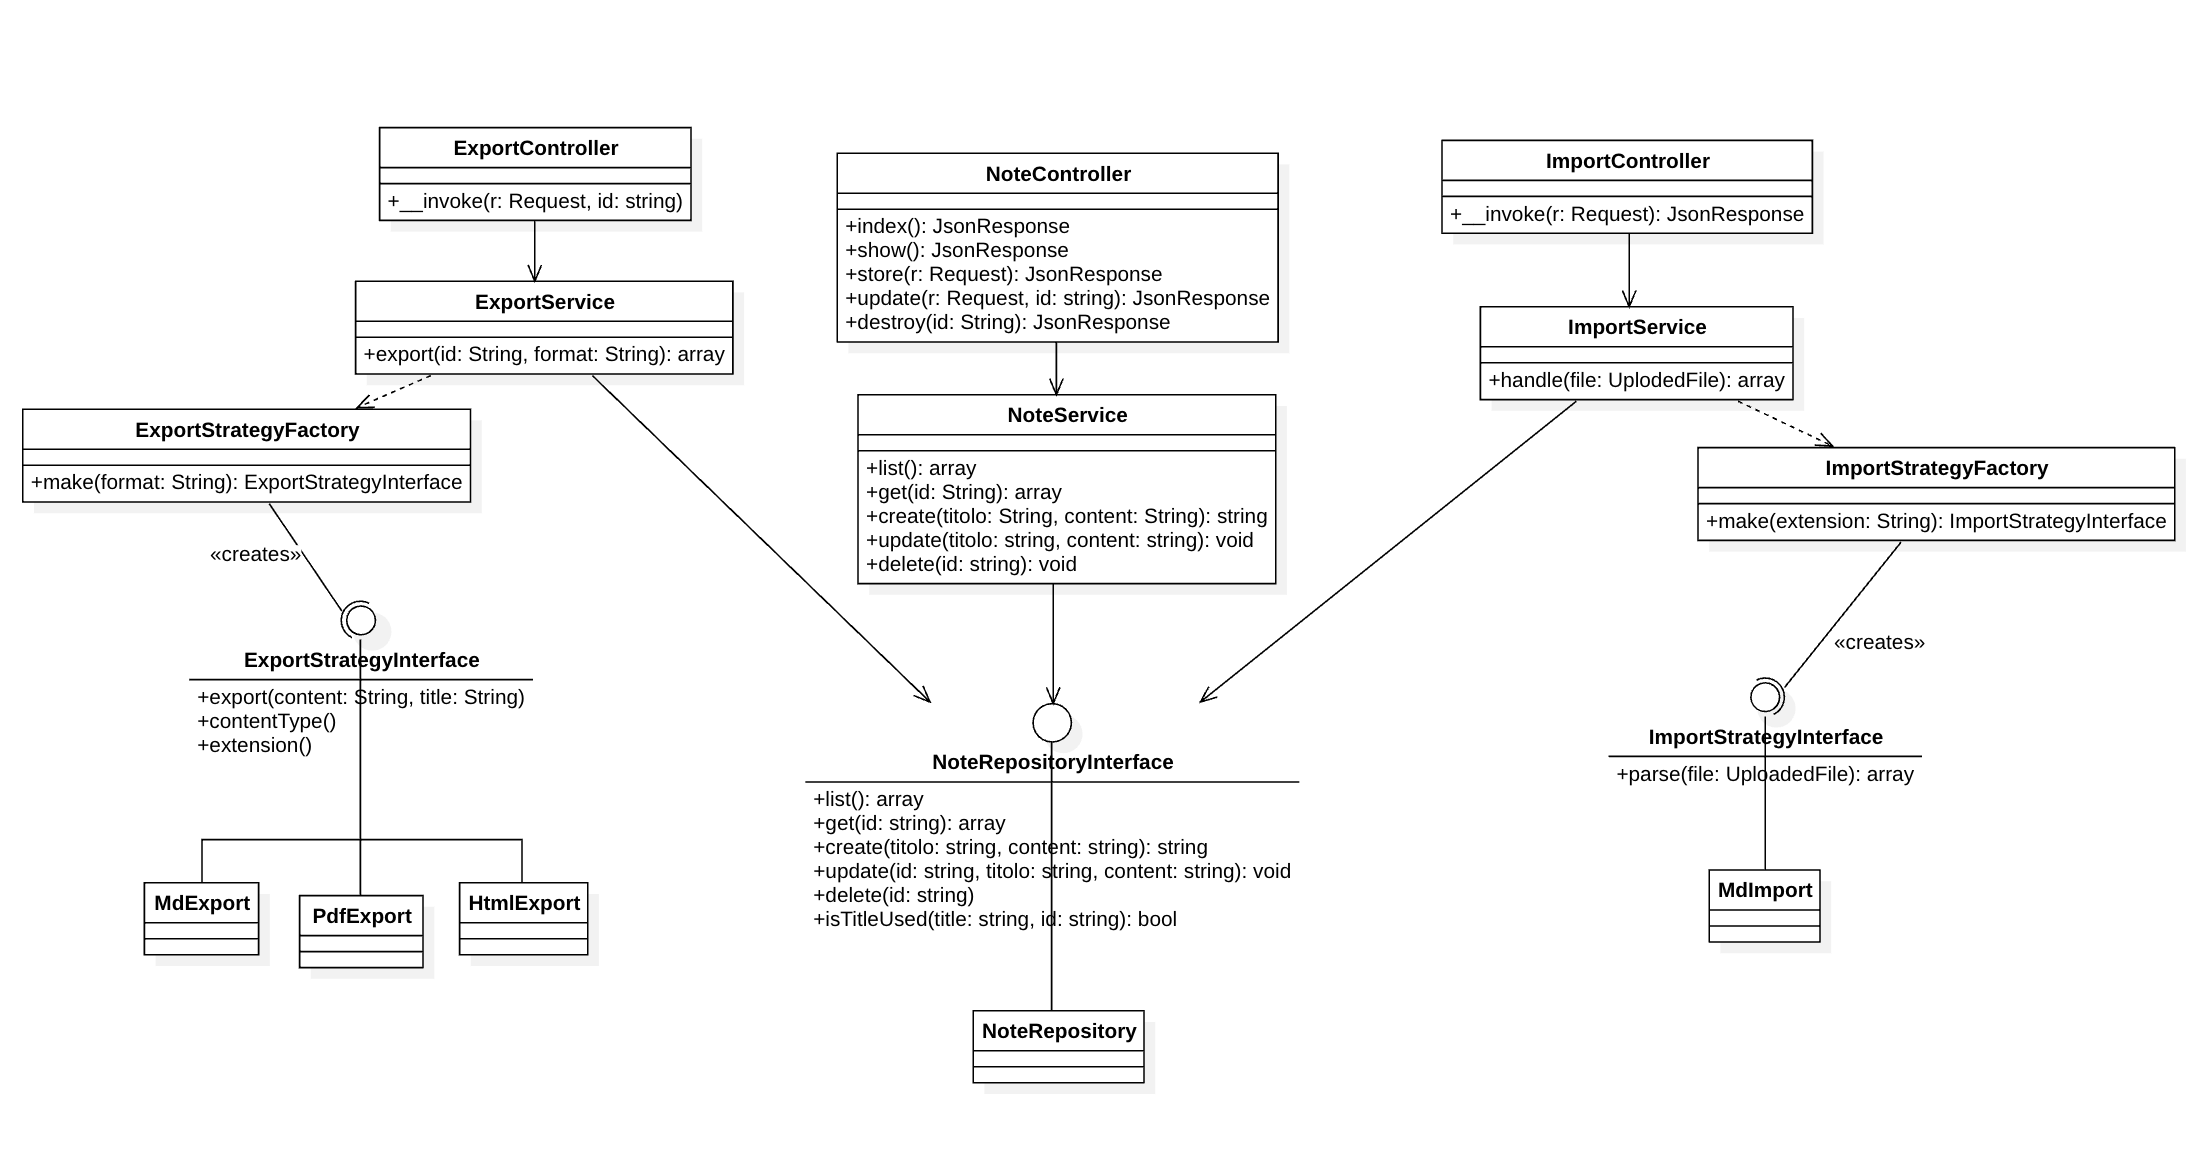
\includegraphics[width=1\textwidth]{resources/Gestione note - Esportazione - Importazione.png}
    \caption{Diagramma delle classi per Gestione note - Esportazione - Importazione}
    \label{fig:gestione-note-esportazione}
\end{figure}
\subparagraph{NoteController}
È il controller HTTP responsabile della gestione delle richieste REST relative alle note. Appartiene al layer di presentazione dell'architettura layered e funge da punto di ingresso per tutte le operazioni CRUD esposte dall'API. Si limita a validare i dati in ingresso, delegare l'elaborazione a \textit{NoteService} e restituire una risposta HTTP appropriata. Segue la descrizione dei metodi:
\begin{itemize}
    \item \texttt{index() : JsonResponse} - gestisce le richieste \texttt{GET /notes}, restituendo la lista completa delle note in formato JSON con status 200, delegando il recupero dei dati a NoteService
    \item  \texttt{show(string \$id) : JsonResponse} - gestisce le richieste \texttt{GET /notes/\{id\}} e restituisce i dettagli di una singola nota identificata dall'id fornito
    \item  \texttt{store(Request \$request) : JsonResponse} -  gestisce le richieste \texttt{POST /notes}, valida i campi, delega a NoteService la creazione e restituisce la nota creata con status 201
    \item \texttt{update(Request \$request, string \$id) : JsonResponse} - gestisce le richieste \texttt{PUT /notes/\{id\}}, valida i campi e delega l'aggiornamento a NoteService, passando l'id e i nuovi dati
    \item \texttt{destroy(string \$id) : JsonResponse} - gestisce le richieste \texttt{DELETE /notes/\{id\}}, delega l'eliminazione a NoteService e restituisce una risposta vuota con status 204 in caso di successo
\end{itemize}
\subparagraph{NoteService} È il service responsabile della logica di business relativa alle note. Appartiene al layer applicativo dell'architettura layered e funge da intermediario tra il controller e il repository. Dipende esclusivamente dall'interfaccia NoteRepositoryInterface, garantendo il rispetto del principio di inversione delle dipendenze. Segue la descrizione dei metodi:
\begin{itemize}
    \item \texttt{list() : array} - restituisce la lista completa delle note, delegando direttamente al repository
    \item \texttt{get(string \$id) : array} - restituisce i dettagli di una singola nota tramite il suo id
    \item \texttt{create(string \$title, string \$contentMd) : array} - gestisce la creazione di una nuova nota, verificando che il titolo non sia già in uso prima di delegare al repository 
    \item \texttt{update(string \$id, string \$title, string \$contentMd) : array} - gestisce l'aggiornamento di una nota esistente; prima di delegare al repository verifica che il titolo non sia già in uso, escludendo dal confronto la nota corrente così che una nota possa essere salvata con il proprio titolo invariato senza incorrere in un falso positivo
    \item \texttt{delete(string \$id) : void} - delega l'eliminazione della nota al repository
\end{itemize}
\subparagraph{NoteRepositoryInterface} Interfaccia che definisce il contratto che ogni implementazione del repository di note deve rispettare. Appartiene al layer di accesso ai dati dell'architettura layered. Dichiarando la dipendenza su questa interfaccia, NoteService può funzionare con qualsiasi implementazione senza richiedere modifiche al codice applicativo. Segue la descrizione dei metodi: 
\begin{itemize}
    \item \texttt{list() : array} - restituisce la lista completa delle note disponibili, ogni elemento dell'array contiene i metadati della nota senza il contenuto completo
    \item \texttt{get(string \$id) : Note} - restituisce i dati completi di una singola nota identificata dall'id fornito
    \item \texttt{create(string \$title, string \$contentMd) : Note} - crea una nuova nota con il titolo e il contenuto Markdown forniti, genera un identificatore e registra il timestamp di creazione
    \item \texttt{update(string \$id, string \$title, string \$contentMd) : Note} - aggiorna il titolo e il contenuto di una nota esistente assieme al timestamp di ultima modifica
    \item \texttt{delete(string \$id) : void} - elimina definitivamente la nota identificata dall'id fornito
    \item \texttt{isTitleUsed(string \$title, ?string \$excludeId = null) : bool} - verifica se un titolo è già utilizzato da un'altra nota; \texttt{excludeId} permette di escludere dal confronto una nota specifica, per evitare che tale nota venga bloccata dal confronto con se stessa
\end{itemize}
\subparagraph{NoteRepository} È l'implementazione concreta di NoteRepositoryInterface che persiste le note come file Markdown sul filesystem locale tramite Laravel Storage. Realizza tutti i metodi dichiarati nell'interfaccia: \texttt{list(), get(), create(), update(), delete(), isTitleUsed()}; per la descrizione della firma e del contratto di ciascun metodo si rimanda alla sezione dedicata all'interfaccia.
\subparagraph{Note} È una classe Model che rappresenta l'entità Nota nel dominio dell'applicazione. Esistono due tipi di metodo:
\begin{itemize}
    \item \texttt{getData() : array} - serializza l'oggetto in array, utile per passare i dati ai layer superiori
    \item getter singoli (\texttt{getId(), getTitle(), ...}) utili quando serve accedere ad una singola proprietà senza serializzare tutto
\end{itemize}
\subparagraph{ImportController} È il controller HTTP responsabile della gestione delle richieste di importazione. Appartiene al layer di presentazione dell'architettura layered ed è implementato come controller invocabile dato che la sua responsabilità è circoscritta ad una sola operazione. Si limita a validare il file, delegare l'importazione a \textit{ImportService} e costruire la risposta HTTP. Segue la descrizione dei metodi:
\begin{itemize}
    \item \texttt{\_\_invoke(Request \$request) : JsonResponse} - valida il parametro (cioè il campo file della richiesta), delega l'importazione a \textit{ImportService}, passando il file caricato; in caso di successo restituisce la nota importata in formato JSON con status 201, altrimenti ritorna una risposta JSON con status 400.
\end{itemize}
\subparagraph{ImportService} È il service responsabile della logica di importazione di una nota. Appartiene al layer applicativo dell'architettura layered. Dipende da NoteRepositoryInterface garantendo il disaccopiamento dall'implementazione del layer di persistenza. Segue la descrizione dei metodi:
\begin{itemize}
    \item \texttt{handleUpload(UploadedFile \$file) : Note} - estrae l'estensione del file caricato, delega la creazione della strategy corretta a ImportStrategyFactory ed invoca sulla strategy il metodo per estrarre il contenuto in Markdown; successivamente aggiunge un timestamp al titolo della nota per evitare conflitti e invoca \texttt{NoteRepositoryInterface::create()}, ritornando un array.
\end{itemize}
\subparagraph{ImportStrategyFactory} - È la factory responsabile della creazione della strategy di importazione corretta in base all'estensione del file caricato. Appartiene al layer applicativo dell'architettura layered e implementa il pattern Factory Method, centralizzando la logica di selezione della stratefy. Segue la descrizione dei metodi:
\begin{itemize}
    \item \texttt{make(string \$extension) : ImportStrategyInterface} - metodo statico che istanzia la strategy concreta corrispondente all'estensione del file caricato.
\end{itemize} 
\subparagraph{ImportStrategyInterface} Interfaccia che definisce il contratto che ogni strategy di importazione deve rispettare. Appartiene al layer applicativo dell'architettura layered e rappresenta il punto di astrazione del pattern strategy applicato all'importazione delle note. Segue la descrizione dei metodi:
\begin{itemize}
    \item \texttt{parse(UploadedFile \$file) : array} - estrae il contenuto in Markdown e il titolo della note dal file caricato.
\end{itemize}
\subparagraph{MdImport} È l'implementazione concreta di ImportStrategyInterface per l'importazione di file \texttt{.md}. Per la descrizione della firma e del contratto di ciascun metodo si rimanda alla sezione dedicata all'interfaccia.

\subparagraph{ExportController} È il controller HTTP responsabile della gestione delle richieste di esportazione, rendendo disponibile una nota come file scaricabile. Appartiene al layer di presentazione dell'architettura layered ed è implementato come controller invocabile dato che la sua responsabilità è circoscritta ad una sola operazione. Si limita a validare il formato richiesto, delega l'esportazione a \textit{ExportService} e costruisce la risposta HTTP con gli header appropriati per il download dei file. Segue la descrizione dei metodi:
\begin{itemize}
    \item \texttt{export(Request \$request, string \$id)} - valida il parametro (cioè il formato con cui si vuole esportare la nota) e delega l'esportazione a \textit{ExportService}, passando l'id della nota e il formato richiesto; in caso di successo restituisce una risposta binaria in modo che il browser tratti la risposta come un file da scaricare, altrimenti ritorna una risposta JSON con status 404
    \item \texttt{exportRaw(Request \$request)} - valida i parametri (cioè il titolo, il contenuto e il formato con cui si vuole esportare la nota) e delega l'esportazione a \textit{ExportService}, passando i diversi parametri e il formato richiesto; in caso di successo restituisce una risposta binaria in modo che il browser tratti la risposta come un file da scaricare, altrimenti ritorna una risposta JSON con status 404
\end{itemize}
\subparagraph{ExportService} È il service responsabile della logica di esportazione di una nota in un formato file. Appartiene al layer applicativo dell'architettura layered e gestisce la collaborazione tra il repository e la factory delle strategy di esportazione. Dipende da NoteRepositoryInterface, garantendo il disaccopiamento dal layer di persistenza. Segue la descrizione dei metodi:
\begin{itemize}
    \item \texttt{export(string \$id, string \$format) : array} - recupera la nota identificata dall'id tramite il repository, delega la creazione della strategy corretta a \textit{ExportStrategyFactory} in base al formato richiesto ed invoca sulla strategy i diversi metodi per ottenere il contenuto del file esportato, il MIME type e l'estensione
    \item \texttt{exportRaw(string \$title, string \$content, string \$format) : array} - delega la creazione della strategy corretta a \textit{ExportStrategyFactory} in base al formato richiesto ed invoca sulla strategy i diversi metodi per ottenere il contenuto del file esportato, il MIME type e l'estensione
\end{itemize}
\subparagraph{ExportStrategyFactory} È la factory responsabile della creazione della strategy di esportazione corretta in base al formato richiesto. Appartiene al layer applicativo dell'architettura layered e implementa il pattern Factory Method, centralizzando la logica di selezione della strategy. Segue la descrizione dei metodi:
\begin{itemize}
    \item \texttt{make(string \$format) : ExportStrategyInterface} - metodo statico che istanzia e restituisce la strategy concreta corrispondente al formato richiesto
\end{itemize}
\subparagraph{ExportStrategyInterface} Interfaccia che definisce il contratto che ogni strategy di esportazione deve rispettare. Appartiene al layer applicativo dell'architettura layered e rappresenta il punto di astrazione del pattern strategy applicato all'esportazione delle note. Segue la descrizione dei metodi:
\begin{itemize}
    \item \texttt{export (string \$content, string \$title) : string} - trasforma il contenuto Markdown della nota nel formato di output specifico della strategy
    \item \texttt{contentType() : string} - restituisce il MIME type associato al formato di esportazione, per consentire al browser di interpretare correttamente il file ricevuto
    \item \texttt{extension() : string} - restituisce l'estensione del file associata al formato di esportazione, utilizzata per costruire il nome del file
\end{itemize}
\subparagraph{MdExport} È l'implementazione concreta di ExportStrategyInterface per l'esportazione nel formato Markdown, è la strategy più semplice del sistema in quanto il contenuto delle note è già nativamente in formato Markdown, quindi non richiede alcuna trasformazione. Per la descrizione della firma e del contratto di ciascun metodo si rimanda alla sezione dedicata all'interfaccia.
\subparagraph{HtmlExport} È l'implementazione concreta di ExportStrategyInterface per l'esportazione nel formato HTML. Utilizza la libreria Parsedown per convertire il contenuto Markdown della nota in markup HTML, che viene poi incorporato in un documento HTML completo e ben formato. Per la descrizione della firma e del contratto di ciascun metodo si rimanda alla sezione dedicata all'interfaccia.
\subparagraph{PdfExport} È l'implementazione concreta di ExportStrategyInterface per l'esportazione nel formato PDF. Prima delega al parser la trasformazione del Markdown in HTML, poi utilizza la libreria \texttt{barryvdh/laravel-domppdf} per convertire l'HTML in un documento PDF binario. Per la descrizione della firma e del contratto di ciascun metodo si rimanda alla sezione dedicata all'interfaccia.
\subparagraph{EditorContentFormatter} Utility dedicata alla conversione di contenuti HTML generati da editor testuali in testo normalizzato in formato Markdown, ha l'obiettivo di eliminare elementi nascosti o metadati che utilizziamo nell'editor per la visualizzazione di blocchi in seguito alla generazione di testo con LLM. Segue la descrizione dei metodi:
\begin{itemize}
    \item \texttt{htmlToMarkdown(string \$html) : string} - riceve in input una stringa contenente HTML e restituisce una versione testuale normalizzata del contenuto
    \item \texttt{nodeToText(DOMNode \$node) : string} - metodo ricorsivo utilizzato per convertire i nodi del DOM in contenuto testuale
    \item \texttt{normalizeMarkdownText(string \$text) : string} - metodo di normalizzazione finale del testo estratto
\end{itemize}

\paragraph{Interazione con LLM}
\vspace{0.5em}
\begin{figure}[H]
    \centering
    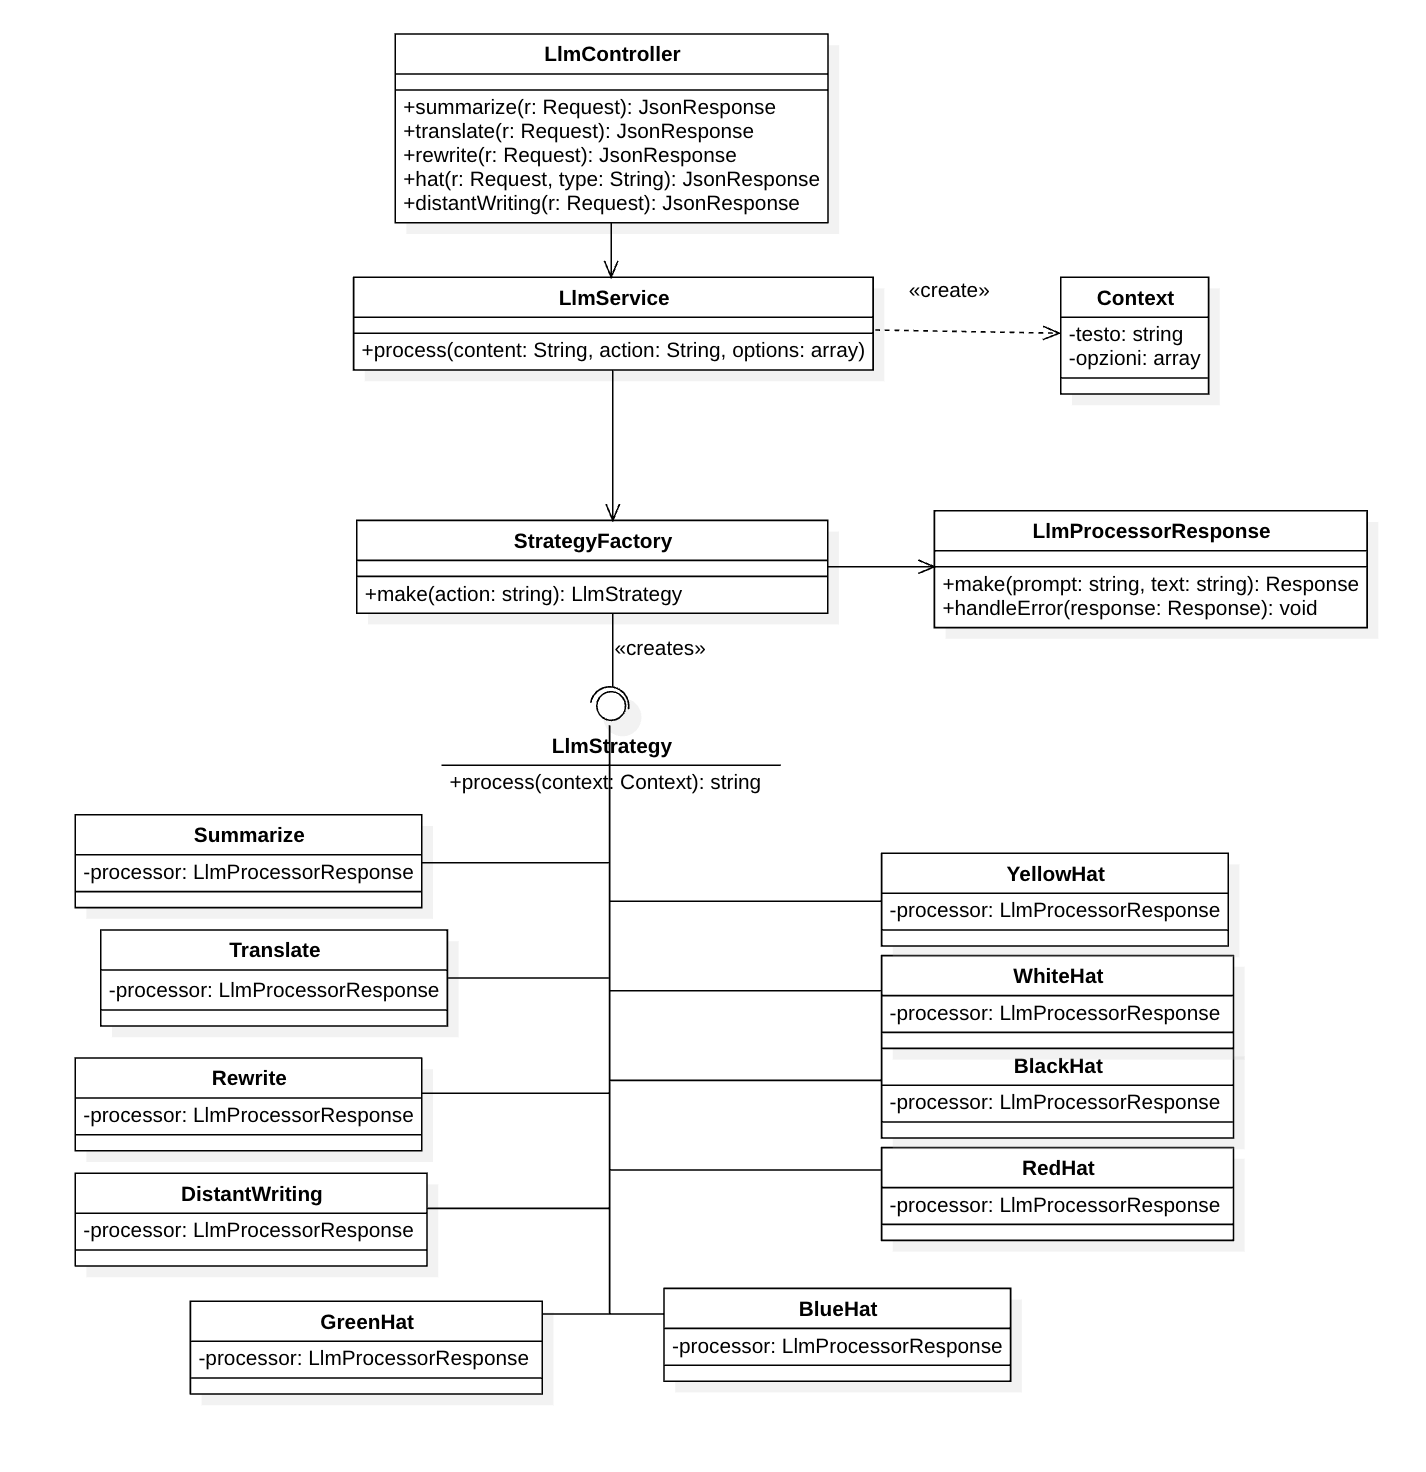
\includegraphics[width=1\textwidth]{resources/Integrazione LLM.png}
    \caption{Diagramma delle classi per Interazione con LLM}
    \label{fig:interazione-llm}
\end{figure}
\subparagraph{LlmController} È il controller HTTP responsabile della gestione delle richieste di elaborazione del testo tramite modelli linguistici. Appartiene al layer di presentazione dell'architettura layered ed è implementato come controller invocabile dato che la sua responsabilità è circoscritta a una sola operazione. Si limita a validare i dati in ingresso, delegare l'elaborazione a \textit{LlmService} e restituire il risultato in formato JSON. Segue la descrizione dei metodi: 
\begin{itemize}
    \item \texttt{\_\_invoke(Request \$request, string \$id) : JsonResponse} - valida i parametri (il content, l'azione da svolgere e i parametri aggiuntivi dipendenti dall'azione), delega l'elaborazione a \textit{LlmService} e restituisce il risultato in una risposta JSON con status 200.
\end{itemize}
\subparagraph{LlmService} È il service responsabile della logica di elaborazione del testo tramite modelli linguistici. Appartiene al layer applicativo dell'architettura layered e gestisce la collaborazione tra \textit{LlmStrategyFactory} e le strategy di elaborazione, che ne eseguono il processo. Si limita a costruire il contesto di esecuzione e delegare il lavoro alle classi di servizio. Segue la descrizione dei metodi:
\begin{itemize}
    \item \texttt{process(string \$content, string \$action, array \$options = []) : string} - costruisce un oggetto \textit{LlmContext} con il testo da elaborare e le opzioni aggiuntive, delega la selezione e creazione della strategy a \textit{LlmStrategyFactory} in base all'azione e esegue la strategia. Infine restituisce il testo prodotto dalla strategy.
\end{itemize}
\subparagraph{LlmStrategyFactory} È la factory responsabile della creazione della strategy di elaborazione testuale, elaborata in base all'azione richiesta. Appartiene al layer applicativo dell'architettura layered e implementa il pattern Factory Method, centralizzando la logica di selezione della strategy. Segue la descrizione dei metodi: 
\begin{itemize}
    \item \texttt{make(string \$action) : LlmStrategyInterface} - metodo statico che istanzia e restituisce la strategy concreta corrispondente all'azione richiesta.
\end{itemize}
\subparagraph{LlmProcessorResponse} Classe utility che gestisce le chiamate a un'API LLM tramite il client HTTP di Laravel. Segue la descrizione dei metodi: 
\begin{itemize}
    \item \texttt{make(string \$prompt, string \$text) : Response} - costruisce e invia una richiesta POST all'endpoint dell'API configurata, restituisce la Response grezza di Laravel
    \item \texttt{handleError(Response \$response) : void} - valida la risposta e lancia una eccezione in caso di errore, se la risposta è andata a buon fine non fa nulla
\end{itemize} 
\subparagraph{LlmStrategyInterface} Interfaccia che definisce il contratto che ogni strategy di eleborazione testuale tramite modelli linguistici deve rispettare. Appartiene al layer applicativo dell'architettura layered e rappresenta il punto di astrazione del pattern strategy applicato alla elaborazione del testo. Segue la descrizione dei metodi: 
\begin{itemize}
    \item \texttt{process(LlmContext \$context) : string} - riceve un oggetto \textit{LlmContext} contenente il testo da elaborare e le opzioni aggiuntive, esegue la chiamata al modello linguistico con il prompt specifico della strategy e restituisce il testo prodotto come string.
\end{itemize}
\subparagraph{LlmContext} È un oggetto di contesto che incapsula i dati necessari all'esecuzione di una strategy di elaborazione testuale; funge da contenitore di informazioni che vengono passata dalla \textit{LlmService} alla strategy selezionata, evitando il passaggio di parametri multipli. Si limita a esporre i dati tramite getter.
\subparagraph{Strategy concrete}
Tutte le strategy implementano \textit{LlmStrategyInterface} e condividono la stessa struttura interna: costruiscono una chiamata all'API del modello linguistico con un prompt specifico per il tipo di richiesta di eleborazione tramite \textit{LlmProcessorResponse} e restituiscono il contenuto generato dal modello. 
\begin{itemize}
    \item \textbf{Summarize} - elabora il testo producendo un riassunto che mantiene solo le informazioni più rilevanti, preservando la voce narrativa originale
    \item \textbf{Translate} - traduce il testo nella lingua specificata tramite il campo dell'array \textit{options} del contesto
    \item \textbf{Rewrite} - riscrive il testo in base alle opzioni scelte dall'utente (variazione stilistica, estensione del testo, correzione grammaticale o miglioramento del lessico)
    \item \textbf{DistantWriting} - genera testo originale a partire da un descrizione fornita dall'utente
    \item \textbf{WhiteHat} - analizza il testo da un punto di vista fattuale, identificando dati oggettivi, informazioni verificabili e lacune conoscitive presenti nel contenuto
    \item \textbf{RedHat} - analizza il testo esprimendo le reazioni emotive e le impressioni intuitive che suscita
    \item \textbf{BlackHat} - individua rischi, criticità, punti deboli e potenziali conseguenze negative presenti nel testo
    \item \textbf{YellowHat} - identifica i punti di forza, benefici e aspetti positivi del testo
    \item \textbf{GreenHat} - propone idee alternative e riformulazioni possibili del contenuto
    \item \textbf{BlueHat} - valuta la chiarezza espositiva e il processo comunicativo del testo, fornendo una riflessione sull'organizzazione del contenuto
\end{itemize}

\subsection{Architettura di deployment}
La scelta della tipologia di \textbf{architettura di deployment} è stata guidata dal contesto di utilizzo del prodotto, dai requisiti di scalabilità previsti dal capitolato e dalle caratteristiche dello stack tecnologico.
Non avendo ricevuto indicazioni specifiche riguardo a vincoli di deployment e non prevedendo significative espansioni o modifiche strutturali, il team ha optato per un'\textbf{architettura monolitica}. Questa soluzione, oltre ad essere in linea con le esigenze del prodotto, semplifica e velocizza la fase di progettazione e sviluppo ed evita la complessità introdotta da un'architettura a microservizi.

\vspace{1em}

Il deployment viene gestito tramite \textbf{Docker Compose} perché, fornendo un ambiente di esecuzione preconfigurato e isolato, si semplificano notevolmente le operazioni di deployment e di manutenzione in qualsiasi ambiente, purché questo supporti Docker, e si evita la necessità di configurazione manuale.

\subsubsection{Organizzazione dei container}
Nonostante l'adozione di un'architettura monolitica dal punto di vista applicativo, il sistema è strutturato in più container al fine di separare le responsabilità tecniche e migliorare la gestione dell'ambiente di esecuzione.
\begin{itemize}
    \item \texttt{app}
        \begin{itemize}
            \item Contiene l'applicazione Laravel
            \item Gestisce la business logic
            \item Interagisce con il database PostgreSQL (opzionale)
        \end{itemize}
    \item \texttt{web}
        \begin{itemize}
            \item Utilizza nginx come web server
            \item Espone l'applicazione sulla porta 8080
            \item Funge da punto di ingresso per le richieste HTTP
            \item Inoltra le richieste al container \texttt{app}
        \end{itemize} 
    \item \texttt{db}
        \begin{itemize}
            \item Utilizza PostgreSQL
            \item Responsabile della persistenza dei dati qualora si opti per questa soluzione invece che per la persistenza su filesystem
        \end{itemize}
    \item \texttt{vite}(sviluppo)
        \begin{itemize}
            \item Esegue un dev server per la compilazione dinamica di JavaScript e CSS
            \item Espone le risorse sulla porta 5173
        \end{itemize}
    \end{itemize}

\subsection{Architettura di dettaglio}

\newpage

\newcounter{RF@O}
\newcounter{RF@D}
\newcounter{RF@OP}

\newcounter{reqTotal}

\newcommand{\reqF}[2]{%
    \refstepcounter{RF@#1}%
    \stepcounter{reqTotal}%
    \noindent{RF-#1-\arabic{RF@#1}}\quad #2\par
}


\section{Stato dei requisiti funzionali}
    
    \begin{longtable}{|l|p{8cm}|p{3.5cm}|}
            \hline
            \textbf{Requisito} & \textbf{Descrizione} & \textbf{Rispettato} \\ \hline
            \endfirsthead
            \hline
            \reqF{O} & Il sistema deve permettere all'utente di visualizzare l'archivio delle note presenti e per ogni nota il suo nome, la data di creazione e la data dell'ultima modifica & NO \\ \hline
            \reqF{O} & Il sistema deve permettere all'utente di aprire una nota & NO \\ \hline
            \reqF{O} & Il sistema deve permettere all'utente di uscire da una nota & NO \\ \hline
            \reqF{O} & Il sistema deve permettere all'utente di creare una nuova nota & NO \\ \hline
            \reqF{O} & Il sistema deve permettere all'utente di salvare la nota su cui sta lavorando & NO \\ \hline
            \reqF{O} & Il sistema deve permettere all'utente di salvare una nota non ancora presente nell'archivio per la prima volta & NO \\ \hline
            \reqF{O} & Il sistema deve permettere all'utente di clonare una nota & NO \\ \hline
            \reqF{O} & Alla clonazione di una nota, il sistema deve assegnare automaticamente un nome di default (es. "Nota \textit{data-ora}") che l’utente può modificare & NO \\ \hline
            \reqF{O} & Il nome di default generato nella clonazione di una nota deve essere univoco all'interno dell'archivio e facilmente riconoscibile all'utente & NO \\ \hline
            \reqF{O} & Il sistema deve permettere all'utente di ricercare le note per nome nell'archivio & NO \\ \hline
            \reqF{O} & Il sistema deve permettere all'utente di eliminare una nota & NO \\ \hline
            \reqF{O} & Il sistema deve permettere all'utente di rinominare una nota & NO \\ \hline
            \reqF{O} & Il sistema deve permettere all'utente di esportare una nota aperta & NO \\ \hline
            \reqF{O} & Il sistema deve permettere all'utente di esportare una nota direttamente dall'archivio & NO \\ \hline
            \reqF{O} & L’esportazione deve preservare integralmente il contenuto testuale della nota, senza perdita o alterazione di caratteri & NO \\ \hline
            \reqF{O} & L’esportazione deve preservare correttamente i caratteri Unicode del testo (es. accenti e simboli), senza sostituzioni o corruzione & NO \\ \hline
            \reqF{O} & Al termine dell’esportazione, il sistema deve notificare esplicitamente l’errore di esportazione all'utente & NO \\ \hline
            \reqF{O} & Il sistema deve permettere all'utente di importare una nota & NO \\ \hline
            \reqF{O} & L’importazione deve preservare integralmente il contenuto testuale della nota, senza perdita o alterazione di caratteri (incl. Unicode) & NO \\ \hline
            \reqF{O} & In caso di file non valido o corrotto, il sistema deve interrompere l’importazione senza creare note parziali e deve notificare chiaramente l’errore all’utente & NO \\ \hline
            \reqF{O} & Il sistema deve permettere all’utente di scrivere nell'editor con caratteri Unicode (es. lettere accentate e simboli) & NO \\ \hline
            \reqF{O} & Il sistema deve compilare la sintassi Markdown  & NO \\ \hline
            \reqF{O} & Il sistema deve permettere la visualizzazione del documento formattato secondo la sintassi Markdown &  NO \\ \hline
            \reqF{O} & L'aggiornamento della visualizzazione formattata deve avvenire in un tempo adeguatamente veloce & NO \\ \hline
            \reqF{O} & Il sistema deve permettere di cambiare modalità di visualizzazione & NO \\ \hline
            \reqF{O} & Il sistema deve fornire un'area di editing di testo in cui è possibile inserire e modificare del testo per la compilazione Markdown & NO \\ \hline
            \reqF{O} & Il sistema deve permettere l'applicazione di formattazioni Markdown senza scrivere manualmente la sintassi & NO \\ \hline
            \reqF{O} & L’editor deve rispondere all’input e alla formattazione dell’utente in modo fluido, senza ritardi percepibili durante la digitazione & NO \\ \hline
            \reqF{O} & Il sistema deve permettere l'applicazione e la rimozione della formattazione testo grassetto senza scrivere manualmente la sintassi & NO \\ \hline
            \reqF{O} & Il sistema deve permettere l'applicazione e la rimozione della formattazione testo corsivo senza scrivere manualmente la sintassi & NO \\ \hline
            \reqF{O} & Il sistema deve permettere l'applicazione e la rimozione della formattazione testo sottolineato senza scrivere manualmente la sintassi & NO \\ \hline
            \reqF{O} & Il sistema deve consentire l’applicazione e la rimozione della formattazione testo barrato senza richiedere l’inserimento manuale della sintassi & NO \\ \hline
            \reqF{O} & Il sistema deve consentire l'inserimento e la rimozione di link ipertestuali senza richiedere l'inserimento manuale della sintassi & NO \\ \hline
            \reqF{O} & L’editor deve rendere i link ipertestuali facilmente riconoscibili (es. evidenziandoli graficamente) e distinguibili dal testo normale & NO \\ \hline
            \reqF{O} & Il sistema deve consentire l'applicazione e la rimozione della formattazione testo commentato senza richiedere l'inserimento manuale della sintassi & NO \\ \hline
            \reqF{O} & Il sistema deve consentire l'inserimento di elenchi numerati & NO \\ \hline
            \reqF{O} & Il sistema deve consentire l'inserimento di elenchi puntati & NO \\ \hline
            \reqF{O} & Il sistema deve permettere all'utente di annullare l'ultima modifica fatta & NO \\ \hline
            \reqF{O} & Il sistema deve permettere all'utente di ripristinare la modifica precedentemente annullata & NO \\ \hline
            \reqF{O} & Il sistema deve permettere all'utente di selezionare porzioni di testo, sia tramite mouse che tastiera & NO \\ \hline
            \reqF{O} & Il sistema deve permettere all'utente di copiare il testo selezionato & NO \\ \hline
            \reqF{O} & Il sistema deve permettere all'utente di tagliare il testo selezionato & NO \\ \hline
            \reqF{O} & L'editor deve poter fare copiare e tagliare all'utente il testo in modo fluido, senza ritardi percepibili & NO \\ \hline
            \reqF{O} & L'editor deve preservare correttamente il contenuto e la struttura del testo copiato e tagliato, senza perdita o alterazioni di caratteri & NO \\ \hline
            \reqF{O} & Il sistema deve permettere all'utente di incollare del testo nell'area di testo & NO \\ \hline
            \reqF{O} & L'editor deve poter fare incollare all'utente il testo in modo fluido, senza ritardi percepibili & NO \\ \hline
            \reqF{O} & L'editor deve preservare e incollare correttamente il contenuto e la struttura del testo, senza perdita o alterazioni di caratteri & NO \\ \hline
            \reqF{O} & Il sistema deve permettere all'utente di esportare una nota aperta in MD & NO \\ \hline
            \reqF{O} & Il sistema deve permettere all'utente di esportare una nota direttamente dall'archivio in MD & NO \\ \hline
            \reqF{O} & Il sistema deve avvisare l'utente della presenza di una nota con lo stesso nome in seguito al primo salvataggio & NO \\ \hline
            \reqF{O} & Il sistema deve permettere all'utente di criticare il testo secondo il modello dei "Sei Cappelli" & NO \\ \hline
            \reqF{O} & Il sistema deve permettere all'utente di criticare il testo con una "Visione Emotiva" (Cappello Rosso) & NO \\ \hline
            \reqF{O} & Il sistema deve permettere all'utente di criticare il testo con una "Visione Neutra" (Cappello Bianco) & NO \\ \hline
            \reqF{O} & Il sistema deve permettere all'utente di criticare il testo con una "Visione Ottimista" (Cappello Giallo) & NO \\ \hline
            \reqF{O} & Il sistema deve permettere all'utente di criticare il testo con una "Visione dell'avvocato del Diavolo" (Cappello Nero) & NO \\ \hline
            \reqF{O} & Il sistema deve permettere all'utente di criticare il testo con una "Visione Originale" (Cappello Verde) & NO \\ \hline
            \reqF{O} & Il sistema deve permettere all'utente di criticare il testo con una "Visione Logica e Strutturata" (Cappello Blu) & NO \\ \hline
            \reqF{O} & Il sistema deve permettere all'utente di riassumere del testo tramite un agente esterno & NO \\ \hline
            \reqF{O} & Il sistema deve permettere all'utente di riscrivere del testo tramite un agente esterno & NO \\ \hline
            \reqF{O} & Il sistema deve permettere all'utente di scegliere il modo in cui verrà riscritto il testo (correzione grammaticale, estensione del testo, miglioramento del lessico, variazione stilistica) & NO   \\ \hline
            \reqF{O} & Il sistema deve permettere all'utente di tradurre del testo tramite un agente esterno & NO \\ \hline
            \reqF{O} & Il sistema deve permettere l'invio da parte dell'utente di un prompt a un agente esterno per la generazione di testo (Distant Writing) & NO \\ \hline
            \reqF{O} & Il sistema deve permettere all'utente di sostituire nell'editor il testo originale con quello generate dall'agente esterno (riassunto, riscrittura, traduzione) & NO \\ \hline
            \reqF{O} & Il sistema deve permettere all'utente di aggiungere nell'editor, in seguito alla selezione del testo originale, quello generato dall'agente esterno (riassunto, riscrittura, traduzione) & NO \\ \hline
            \reqF{O} & Il sistema deve permettere all'utente di aggiungere nell'editor, in coda a tutto il testo presente nell'editor, quello generato dall'agente esterno (riassunto, riscrittura, traduzione) & NO \\ \hline
            \reqF{O} & Il sistema deve permettere all'utente di "rifiutare" il testo generato dall'agente esterno (riassunto, riscrittura, traduzione) & NO \\ \hline
            \reqF{O} & Il sistema deve permettere all'utente di copiare negli appunti il testo generato dall'agente esterno (riassunti, riscrittura, traduzione, generazione) & NO \\ \hline
            \reqF{O} & L'agente esterno deve produrre testo grammaticalmente, sintatticamente e semanticamente corretto & NO \\ \hline
            \reqF{O} & Il sistema deve avvisare l'utente in caso dell'impossibilità nell'eseguire una richiesta & NO  \\ \hline
            \reqF{O} & Il sistema deve commentare il testo selezionato dall’utente utilizzato per interrogare la generazione (Distant Writing) & NO \\ \hline
            \reqF{O} & Se l’utente aggiunge una traduzione a una parte del testo selezionato, il sistema deve avvisarlo ogni volta che il testo tradotto viene modificato & NO \\ \hline
            \reqF{O} & Il sistema deve consentire all’utente di aggiornare una traduzione precedentemente inserita se il testo originale è presente ed è stato modificato & NO \\ \hline
            \reqF{O} & Il sistema deve consentire all'utente di rimuovere una traduzione precedentemente inserita & NO \\ \hline
            \reqF{O} & Il sistema deve consentire all'utente di rimuovere il testo originale di una traduzione precedentemente inserita & NO \\ \hline
            \reqF{O} & Il sistema deve notificare all'utente la perdita del testo originale di riferimento qualora venga eliminato, lasciando la traduzione priva di collegamento & NO \\ \hline
            \reqF{O} & Il sistema non deve consentire l'inserimento di una traduzione all'interno di una porzione di testo già tradotta & NO \\ \hline
            \reqF{O} & L'agente deve produrre traduzioni corrette nella lingua selezionata & NO \\ \hline
            \reqF{O} & Il sistema alla chiusura di una nota, se presenti delle modifiche non salvate deve avvisare l'utente della presenza di modifiche & NO \\ \hline
            \reqF{O} & Il sistema in caso di problemi di connessione con l'agente esterno deve avvisare l'utente & NO  \\ \hline
            \reqF{O} & Durante una richiesta alla LLM, il sistema deve fornire all’utente un feedback chiaro sullo stato dell’operazione (es. indicatore di caricamento/elaborazione) fino al completamento o alla segnalazione di errore & NO \\ \hline
            \reqF{O} & Il feedback sullo stato della comunicazione con la LLM deve essere non bloccante e deve evitare che l’utente avvii richieste duplicate inconsapevolmente & NO\\ \hline
            \reqF{O} & Il sistema deve permettere all'utente di visualizzare l'editor con il contenuto della nota dopo l'apertura di questa & NO \\ \hline
            \reqF{O} & Il sistema deve avvisare l'utente in caso di tentativo di apertura di una nota non più esistente & NO \\ \hline
            \reqF{O} & Il sistema deve avvisare l'utente in caso di fallimento dell'apertura di una nota a causa di problemi di connessione al server & NO \\ \hline
            \reqF{O} & In caso di tentativo di chiusura di una nota con modifiche non salvate, il sistema deve avvisare l'utente e chiedere se desidera salvare le modifiche prima di chiudere & NO \\ \hline
            \reqF{O} & Il sistema deve permettere all'utente di salvare le modifiche effettuate all'interno di una nota & NO \\ \hline
            \reqF{O} & Il sistema deve avvisare l'utente in caso di presenza di una versione più recente della nota aperta nell'archivio & NO \\ \hline
            \reqF{O} & Il sistema deve permettere all'utente di sovrascrivere la nota presente nell'archivio con la versione aperta in caso di conflitto di versioni & NO \\ \hline
            \reqF{O} & Il sistema deve permettere all'utente di salvare la nota aperta con un nuovo nome in caso di conflitto con la versione presente nell'archivio & NO \\ \hline
            \reqF{O} & Il sistema deve permettere all'utente di aggiornare la nota aperta con le modifiche presenti nella versione più recente nell'archivio in caso di conflitto di versioni & NO \\ \hline
            \reqF{O} & Il sistema deve avvisare l'utente in caso di errori durante il salvataggio della nota causati da problemi di connessione al server & NO \\ \hline
            \reqF{O} & Il sistema deve avvisare l'utente in caso di tentativo di clonazione di una nota non più esistente & NO \\ \hline
            \reqF{O} & Il sistema deve avvisare in caso di impossibilità di clonare una nota a causa di problemi di connessione al server & NO \\ \hline
            \reqF{O} & Il sistema deve chiedere all'utente di confermare l'eliminazione di una nota & NO \\ \hline
            \reqF{O} & Il sistema deve avvisare l'utente in caso di impossibilità di eliminazione di una nota a causa di problemi di connessione al server & NO \\ \hline
            \reqF{O} & Il sistema deve impedire all'utente di rinominare una nota con un nome già presente nell'archivio e visualizzare un messaggio di errore & NO \\ \hline
            \reqF{O} & Il sistema deve avvisare l'utente in caso di impossibilità di rinominare una nota a causa di problemi di connessione al server & NO \\ \hline
            \reqF{O} & Il sistema deve avvisare l'utente in caso di impossibilità di esportare una nota a causa di problemi di connessione al server & NO \\ \hline
            \reqF{O} & Il sistema deve dare la possibilità all'utente di importare una nota in formato MD & NO \\ \hline
            \reqF{O} & Il sistema deve avvisare l'utente in caso di problemi di connessione al server durante l'importazione di una nota & NO \\ \hline
            \reqF{O} & Il sistema deve permettere all'utente di inserire elementi in un elenco puntato o numerato & NO \\ \hline
            \reqF{O} & Il sistema deve permettere all'utente di rimuovere elementi da un elenco puntato o numerato & NO \\ \hline
            \reqF{O} & Il sistema deve avvisare l'utente in caso di problemi di connessione con l'agente esterno durante la ritraduzione di una porzione di testo precedentemente tradotta & NO \\ \hline
            \reqF{D} & Il sistema deve aggiornare automaticamente i risultati della ricerca ad ogni modifica dell’input di ricerca & NO \\ \hline
            \reqF{D} & Il sistema deve permettere all'utente di esportare una nota aperta in PDF & NO \\ \hline
            \reqF{D} & Il sistema deve permettere all'utente di esportare una nota aperta in HTML & NO \\ \hline
            \reqF{D} & Il sistema deve permettere all'utente di esportare una nota direttamente dall'archivio in PDF & NO \\ \hline
            \reqF{D} & Il sistema deve permettere all'utente di esportare una nota direttamente dall'archivio in HTML & NO \\ \hline
            \reqF{D} & Il sistema deve permettere all'utente di utilizzare scorciatoie da tastiera per formattare il testo & NO \\ \hline
            \reqF{D} & Il sistema deve comunicare all'utente eventuali errori grammaticali nell'editor & NO \\ \hline
            \reqF{D} & Il sistema deve consentire all’utente di eseguire un minimo di 20 operazioni consecutive di annullamento e di ripristino delle modifiche sull’editor della nota corrente & NO \\ \hline
            \reqF{D} & In caso di incollaggio di contenuti non testuali, l’editor deve mantenere la reattività e mostrare una notifica non bloccante che spieghi l’azione effettuata (rifiuto o conversione in testo) & NO \\ \hline
            \reqF{D} & L'archivio deve aggiornarsi dinamicamente con i risultati della ricerca ad ogni modifica dell’input con una risposta percepita come immediata dall’utente &  NO \\ \hline
            \reqF{D} & L'editor deve evidenziare in modo chiaro e distinguibile la porzione di testo utilizzato come prompt per l'interrogazione del LLM, così da renderla immediatamente riconoscibile all'utente & NO \\ \hline
            \reqF{D} & L’aggiornamento della visualizzazione formattata non deve bloccare l’input dell’utente durante la digitazione & NO \\ \hline
            \reqF{OP} & Il sistema deve aggiornare automaticamente la visualizzazione del testo formattato ad ogni modifica del Markdown, senza richiedere un’azione esplicita & NO \\ \hline
            \reqF{OP} & Il sistema deve comunicare all'utente eventuali errori di sintassi nei marcatori nell'editor & NO \\ \hline
            \reqF{OP} & L'editor deve permettere all'utente di interagire direttamente con la LLM tramite marcatori & NO \\ \hline
            \reqF{OP} & Il sistema deve permettere all'utente di registrarsi tramite nome utente e password & NO \\ \hline
            \reqF{OP} & Se password o nome utente non sono corrette il sistema non deve permettere la registrazione & NO \\ \hline
            \reqF{OP} & Il sistema deve permettere all'utente di accedere al proprio account & NO \\ \hline
            \reqF{OP} & Se password o nome utente non sono corrette il sistema non deve permettere l'autenticazione & NO \\ \hline
            \reqF{OP} & L'utente può effettuare il logout e terminare la sessione & NO \\ \hline
            \reqF{OP} & Il sistema deve permettere ad un utente autenticato di eliminare il proprio account  & NO \\ \hline
            \reqF{OP} & Il sistema deve richiedere la password dell'utente per l'eliminazione del suo account  & NO \\ \hline
            \reqF{OP} & Il sistema deve avvisare l'utente che la password inserita per l'eliminazione dell'account è sbagliata  & NO \\ \hline
            \reqF{OP} & Il sistema deve richiedere la conferma all'utente per l'eliminazione del suo account  & NO \\ \hline
            \reqF{OP} & Il sistema deve permettere all'utente autenticato di salvare note nel proprio account & NO \\ \hline
            \reqF{OP} & Il sistema deve permettere all'utente autenticato di aprire una delle note salvate nel proprio account & NO \\ \hline
            \reqF{OP} & Il sistema durante il salvataggio, nel caso in cui il DataBase non sia raggiungibile, deve visualizzare un messaggio d'errore & NO \\ \hline
            \reqF{OP} & Il sistema durante l'apertura di una nota, nel caso in cui il DataBase non sia raggiungibile, deve visualizzare un messaggio d'errore & NO \\ \hline
            \reqF{OP} & Le credenziali dell'utente devono essere trasmesse in modo sicuro durante l'autenticazione e la registrazione & NO \\ \hline
            \reqF{OP} & Il sistema deve completare una richiesta di autenticazione e registrazione in un breve lasso di tempo & NO\\ \hline
            \reqF{OP} & Il sistema non deve memorizzare né mostrare password in chiaro & NO \\ \hline
            \reqF{OP} & Il sistema deve limitare ad un massimo di 3 tentativi di accesso falliti per ridurre il rischio di attacchi a forza bruta & NO \\ \hline
            \reqF{OP} & In caso di credenziali errate, il messaggio di errore non deve rivelare se sia il nome utente o la password ad essere errata & NO \\ \hline
            \reqF{OP} & I messaggi di errore in autenticazione e registrazione devono essere chiari e indicare all’utente come correggere l’input & NO \\ \hline
            \reqF{OP} & I campi di inserimento credenziali devono fornire feedback immediato su validità del formato (es. vincoli su nome utente/password), senza attendere l’invio del form & NO \\ \hline
            \reqF{OP} & Dopo l’autenticazione, la sessione deve scadere automaticamente dopo un periodo di inattività pari a 1 mese & NO \\ \hline
            \reqF{OP} & Il sistema deve avvisare l'utente in caso di mancata registrazione/autenticazione dovuta a problemi di connessione al server & NO \\ \hline
            \reqF{OP} & Il sistema deve avvisare l'utente in caso di impossibilità di eliminazione dell'account a causa di problemi di connessione al server & NO \\ \hline
            \caption{Tabella Requisiti Funzionali}
        \end{longtable}

\end{document}

